% remove "answers" to suppress solutions
\documentclass[11pt,addpoints,answers]{exam}

\usepackage{fullpage}
\usepackage{amsfonts, amsmath, amssymb, amsthm}
\usepackage{mathtools}
\usepackage{enumerate}
\usepackage{listings}
\usepackage[boxed]{algorithm}
\usepackage[noend]{algpseudocode}

\usepackage{hyperref}
\usepackage{tikz}
\usetikzlibrary{positioning}
\usepackage[inline,shortlabels]{enumitem}
\usetikzlibrary{automata, positioning, arrows}
\usepackage{subcaption}

% in order to compile this file you need to get 'header.tex' from
% Canvas and change the line below to the appropriate file path
%%% theorems

\theoremstyle{plain}            % following are "theorem" style
\newtheorem{theorem}{Theorem}[section]
\newtheorem{lemma}[theorem]{Lemma}
\newtheorem{corollary}[theorem]{Corollary}
\newtheorem{proposition}[theorem]{Proposition}
\newtheorem{claim}[theorem]{Claim}
\newtheorem{fact}[theorem]{Fact}
\newtheorem{openproblem}[theorem]{Open Problem}

\theoremstyle{definition}       % following are def style
\newtheorem{definition}[theorem]{Definition}
\newtheorem{conjecture}[theorem]{Conjecture}
\newtheorem{example}[theorem]{Example}
\newtheorem{protocol}[theorem]{Protocol}
\newtheorem{exercise}[theorem]{Exercise}

\theoremstyle{remark}           % following are remark style
\newtheorem{remark}[theorem]{Remark}
\newtheorem{note}[theorem]{Note}
\newtheorem*{aside}{Aside}
\newtheorem*{gn}{Grading Note} % grading note

%%% special sets
\newcommand{\bit}{\ensuremath{\{0,1\}}}
\newcommand{\bitt}{\ensuremath{\{-1,1\}}}

% font for general-purpose algorithms
\newcommand{\algo}[1]{\ensuremath{\mathsf{#1}}}
% font for general-purpose computational problems
\newcommand{\problem}[1]{\ensuremath{\mathsf{#1}}}
% font for complexity classes
%\newcommand{\class}[1]{\ensuremath{\mathsf{#1}}}

\global\long\def\path{\mathrm{path}}
% asymptotics
%\DeclareMathOperator{\poly}{poly}
%\DeclareMathOperator{\polylog}{polylog}
\DeclareMathOperator{\negl}{negl}
\DeclareMathOperator{\Otil}{\tilde{O}}
\DeclareMathOperator{\Ostar}{O^*}

%%% "LEFT-RIGHT" PAIRS OF SYMBOLS

% inner product
\DeclarePairedDelimiter\inner{\langle}{\rangle}
% absolute value
\DeclarePairedDelimiter\abs{\lvert}{\rvert}
% a set
\DeclarePairedDelimiter\set{\{}{\}}
% parens
\DeclarePairedDelimiter\parens{(}{)}
% tuple, alias for parens
\DeclarePairedDelimiter\tuple{(}{)}
% square brackets
\DeclarePairedDelimiter\bracks{[}{]}
% rounding off
\DeclarePairedDelimiter\round{\lfloor}{\rceil}
% floor function
\DeclarePairedDelimiter\floor{\lfloor}{\rfloor}
% ceiling function
\DeclarePairedDelimiter\ceil{\lceil}{\rceil}
% length of some vector, element
\DeclarePairedDelimiter\length{\lVert}{\rVert}
% norm
\DeclarePairedDelimiter\norm{\lVert}{\rVert}
% length (as a string)
\DeclarePairedDelimiter\len{\lvert}{\rvert}
% bra-kets
\DeclarePairedDelimiter\bra{\langle}{\rvert}
\DeclarePairedDelimiter\ket{\lvert}{\rangle}
\newcommand{\braket}[2]{\ensuremath{\langle #1 \vert #2 \rangle}}
\newcommand{\ketbra}[2]{\ensuremath{\lvert #1 \rangle \langle #2 \rvert}}

%%% MATH OPERATORS
\DeclareMathOperator{\Var}{Var}
\DeclareMathOperator{\tr}{Tr}
\DeclareMathOperator{\supp}{supp}
\DeclareMathOperator{\var}{var}
\DeclareMathOperator{\vol}{vol}
\DeclareMathOperator{\sign}{sign}

%%% BLACKBOARD SYMBOLS

\newcommand{\C}{\ensuremath{\mathbb{C}}}
\newcommand{\D}{\ensuremath{\mathbb{D}}}
\newcommand{\F}{\ensuremath{\mathbb{F}}}
\newcommand{\G}{\ensuremath{\mathbb{G}}}
\newcommand{\J}{\ensuremath{\mathbb{J}}}
\newcommand{\N}{\ensuremath{\mathbb{N}}}
\newcommand{\Q}{\ensuremath{\mathbb{Q}}}
\newcommand{\R}{\ensuremath{\mathbb{R}}}
\newcommand{\T}{\ensuremath{\mathbb{T}}}
\newcommand{\Z}{\ensuremath{\mathbb{Z}}}
\newcommand{\QR}{\ensuremath{\mathbb{QR}}}

% sets in calligraphic type

\newcommand{\calD}{\ensuremath{\mathcal{D}}}
\newcommand{\calF}{\ensuremath{\mathcal{F}}}
\newcommand{\calG}{\ensuremath{\mathcal{G}}}
\newcommand{\calH}{\ensuremath{\mathcal{H}}}
\newcommand{\calI}{\ensuremath{\mathcal{I}}}
\newcommand{\calL}{\ensuremath{\mathcal{L}}}
\newcommand{\calN}{\ensuremath{\mathcal{N}}}
\newcommand{\calP}{\ensuremath{\mathcal{P}}}
\newcommand{\calS}{\ensuremath{\mathcal{S}}}
\newcommand{\calX}{\ensuremath{\mathcal{X}}}
\newcommand{\calY}{\ensuremath{\mathcal{Y}}}

% matrices and vectors

\newcommand{\matA}{\ensuremath{\mathbf{A}}}
\newcommand{\matB}{\ensuremath{\mathbf{B}}}
\newcommand{\matC}{\ensuremath{\mathbf{C}}}
\newcommand{\matD}{\ensuremath{\mathbf{D}}}
\newcommand{\matE}{\ensuremath{\mathbf{E}}}
\newcommand{\matF}{\ensuremath{\mathbf{F}}}
\newcommand{\matG}{\ensuremath{\mathbf{G}}}
\newcommand{\matH}{\ensuremath{\mathbf{H}}}
\newcommand{\matI}{\ensuremath{\mathbf{I}}}
\newcommand{\matJ}{\ensuremath{\mathbf{J}}}
\newcommand{\matK}{\ensuremath{\mathbf{K}}}
\newcommand{\matL}{\ensuremath{\mathbf{L}}}
\newcommand{\matM}{\ensuremath{\mathbf{M}}}
\newcommand{\matN}{\ensuremath{\mathbf{N}}}
\newcommand{\matO}{\ensuremath{\mathbf{O}}}
\newcommand{\matP}{\ensuremath{\mathbf{P}}}
\newcommand{\matQ}{\ensuremath{\mathbf{Q}}}
\newcommand{\matR}{\ensuremath{\mathbf{R}}}
\newcommand{\matS}{\ensuremath{\mathbf{S}}}
\newcommand{\matT}{\ensuremath{\mathbf{T}}}
\newcommand{\matU}{\ensuremath{\mathbf{U}}}
\newcommand{\matV}{\ensuremath{\mathbf{V}}}
\newcommand{\matW}{\ensuremath{\mathbf{W}}}
\newcommand{\matX}{\ensuremath{\mathbf{X}}}
\newcommand{\matY}{\ensuremath{\mathbf{Y}}}
\newcommand{\matZ}{\ensuremath{\mathbf{Z}}}
\newcommand{\matzero}{\ensuremath{\mathbf{0}}}

\newcommand{\veca}{\ensuremath{\mathbf{a}}}
\newcommand{\vecb}{\ensuremath{\mathbf{b}}}
\newcommand{\vecc}{\ensuremath{\mathbf{c}}}
\newcommand{\vecd}{\ensuremath{\mathbf{d}}}
\newcommand{\vece}{\ensuremath{\mathbf{e}}}
\newcommand{\vecf}{\ensuremath{\mathbf{f}}}
\newcommand{\vecg}{\ensuremath{\mathbf{g}}}
\newcommand{\vech}{\ensuremath{\mathbf{h}}}
\newcommand{\veck}{\ensuremath{\mathbf{k}}}
\newcommand{\vecm}{\ensuremath{\mathbf{m}}}
\newcommand{\vecp}{\ensuremath{\mathbf{p}}}
\newcommand{\vecq}{\ensuremath{\mathbf{q}}}
\newcommand{\vecr}{\ensuremath{\mathbf{r}}}
\newcommand{\vecs}{\ensuremath{\mathbf{s}}}
\newcommand{\vect}{\ensuremath{\mathbf{t}}}
\newcommand{\vecu}{\ensuremath{\mathbf{u}}}
\newcommand{\vecv}{\ensuremath{\mathbf{v}}}
\newcommand{\vecw}{\ensuremath{\mathbf{w}}}
\newcommand{\vecx}{\ensuremath{\mathbf{x}}}
\newcommand{\vecy}{\ensuremath{\mathbf{y}}}
\newcommand{\vecz}{\ensuremath{\mathbf{z}}}
\newcommand{\veczero}{\ensuremath{\mathbf{0}}}
\newcommand{\vecone}{\ensuremath{\mathbf{1}}}

%%% misc

\newcommand{\eps}{\varepsilon}

%%% for homework and section notes

\newcommand{\commonheader}[2]{
    \pagestyle{headandfoot}
    \setlength{\headheight}{26pt}
    \setlength{\headsep}{16pt}

    \header
        {\small{\textbf{EECS 376: Foundations of Computer Science}} \\ \footnotesize{\textbf{University of Michigan, Spring 2024}}}
        {#1}
        {#2}

    \firstpageheadrule
    \runningheadrule

    \footer
        {}
        {\thepage}
        {}
}

\newcommand{\hwheader}{
    \commonheader
        {\Large \textbf{Homework \hwnum}}
        {\small \textbf{Due 8:00pm, \duedate\\ {\tiny(accepted until 9:59 pm, no credit after)}}}
}

\newcommand{\hwslnheader}{
    \commonheader
    	{}
        {\Large \textbf{Solutions to Homework \hwnum}}
    \printanswers
}

\newcommand{\notesheader}{
    \commonheader
    	{}
        {\Large \textbf{Discussion Notes \sectionnum}}
}

\newcommand{\practiceheader}{
    \commonheader
    	{}
        {\Large \textbf{Discussion Worksheet \sectionnum}}
}

\newcommand{\practiceslnheader}{
    \commonheader
    	{}
        {\Large \textbf{Solutions to Discussion Worksheet \sectionnum}}
}

\newcommand{\reviewheader}{
    \commonheader 
    \smallskip
    	{}
        {\Large \textbf{Midterm Review Notes}}
}

\newcommand{\hwpreface}{

\noindent This homework has \numquestions\ questions, for a total of \numpoints\ points and \numbonuspoints\ extra-credit points.

\noindent Unless otherwise stated, each question requires \emph{clear}, \emph{logically correct}, and \emph{sufficient} justification to convince the reader.

\noindent For bonus/extra-credit questions, we will provide very limited guidance in office hours and on Piazza, and we do not guarantee anything about the difficulty of these questions.
 
\noindent We strongly encourage you to typeset your solutions in \LaTeX.

\noindent If you collaborated with someone, you must state their name(s). You must \emph{write your own solution} for all problems and \emph{may not use any other student’s write-up}.
}

\newcommand{\hint}[1]{
\emph{Hint}: #1
}
\newcommand{\bonus}{
\emph{Optional bonus}:
}
\newcommand{\extracredit}{
\emph{Extra credit}: 
}


\algnewcommand{\algorithmiconinput}[2]{\text{#1 = ``on input #2:}}

% P, NP, NP-Hard, NP-Complete, poly-reduction
\newcommand{\NP}{\textsf{NP}}
\renewcommand{\P}{\textsf{P}}
\newcommand{\NPHard}{\NP\text{-Hard}}
\newcommand{\NPComplete}{\NP\text{-Complete}}
\newcommand{\ptimemap}{\leq_p}

% Languages in this HW
\newcommand{\VC}{\text{VertexCover}}
\newcommand{\DeliveryRoute}{\textsc{Delivery-Route}}
\newcommand{\fSetCov}{\textsc{$f$-SetCover}}
\newcommand{\SetCov}{\textsc{SetCover}}
\newcommand{\VertCov}{\textsc{VertexCover}}
\newcommand{\MaxCut}{\textsc{MaxCut}}

% Approximation commands
\newcommand{\OPT}{\text{OPT}}
\newcommand{\ALG}{\text{ALG}}
\renewcommand{\epsilon}{\varepsilon}
\DeclareMathOperator{\Ex}{\mathbb{E}}

\newcommand{\hwnum}{5}
\newcommand{\duedate}{June 24}
\usepackage{xcolor}

\hwheader   % header for homework

% Comment the following line in order to hide solutions.
% Uncomment the line to show solutions written inside of
% LaTeX solution environments like:
%   \begin{solution}
%     My solution.
%   \end{solution}.

\begin{document}

\hwpreface

\pointsinmargin
\pointpoints{pt}{pts}
\bonuspointpoints{EC pt}{EC pts}
\marginpointname{ \points}
\marginbonuspointname{ \bonuspoints}

\begin{questions}
    \addtocounter{question}{-1}
    
    \question[0] \textbf{Before you start; before you submit.}
    
    If applicable, state the name(s) and uniqname(s) of your collaborator(s).
    
    \begin{solution}
    None.
    \end{solution}
    
    \question[10] \textbf{Self assessment.}
    
    Carefully read and understand the posted solutions to the previous homework. Identify one part for which your own solution has the most room for improvement (e.g., has unsound reasoning, doesn’t show what was required, could be significantly clearer or better organized, etc.). Copy or screenshot this solution, then in a few sentences, explain what was deficient and how it could be fixed.
    
    (Alternatively, if you think one of your solutions is significantly \emph{better} than the posted one, copy it here and explain why you think it is better.)
    
    You may reference the answer key, but your answer should be in your own words.
    
    \begin{solution}
    \begin{center}
      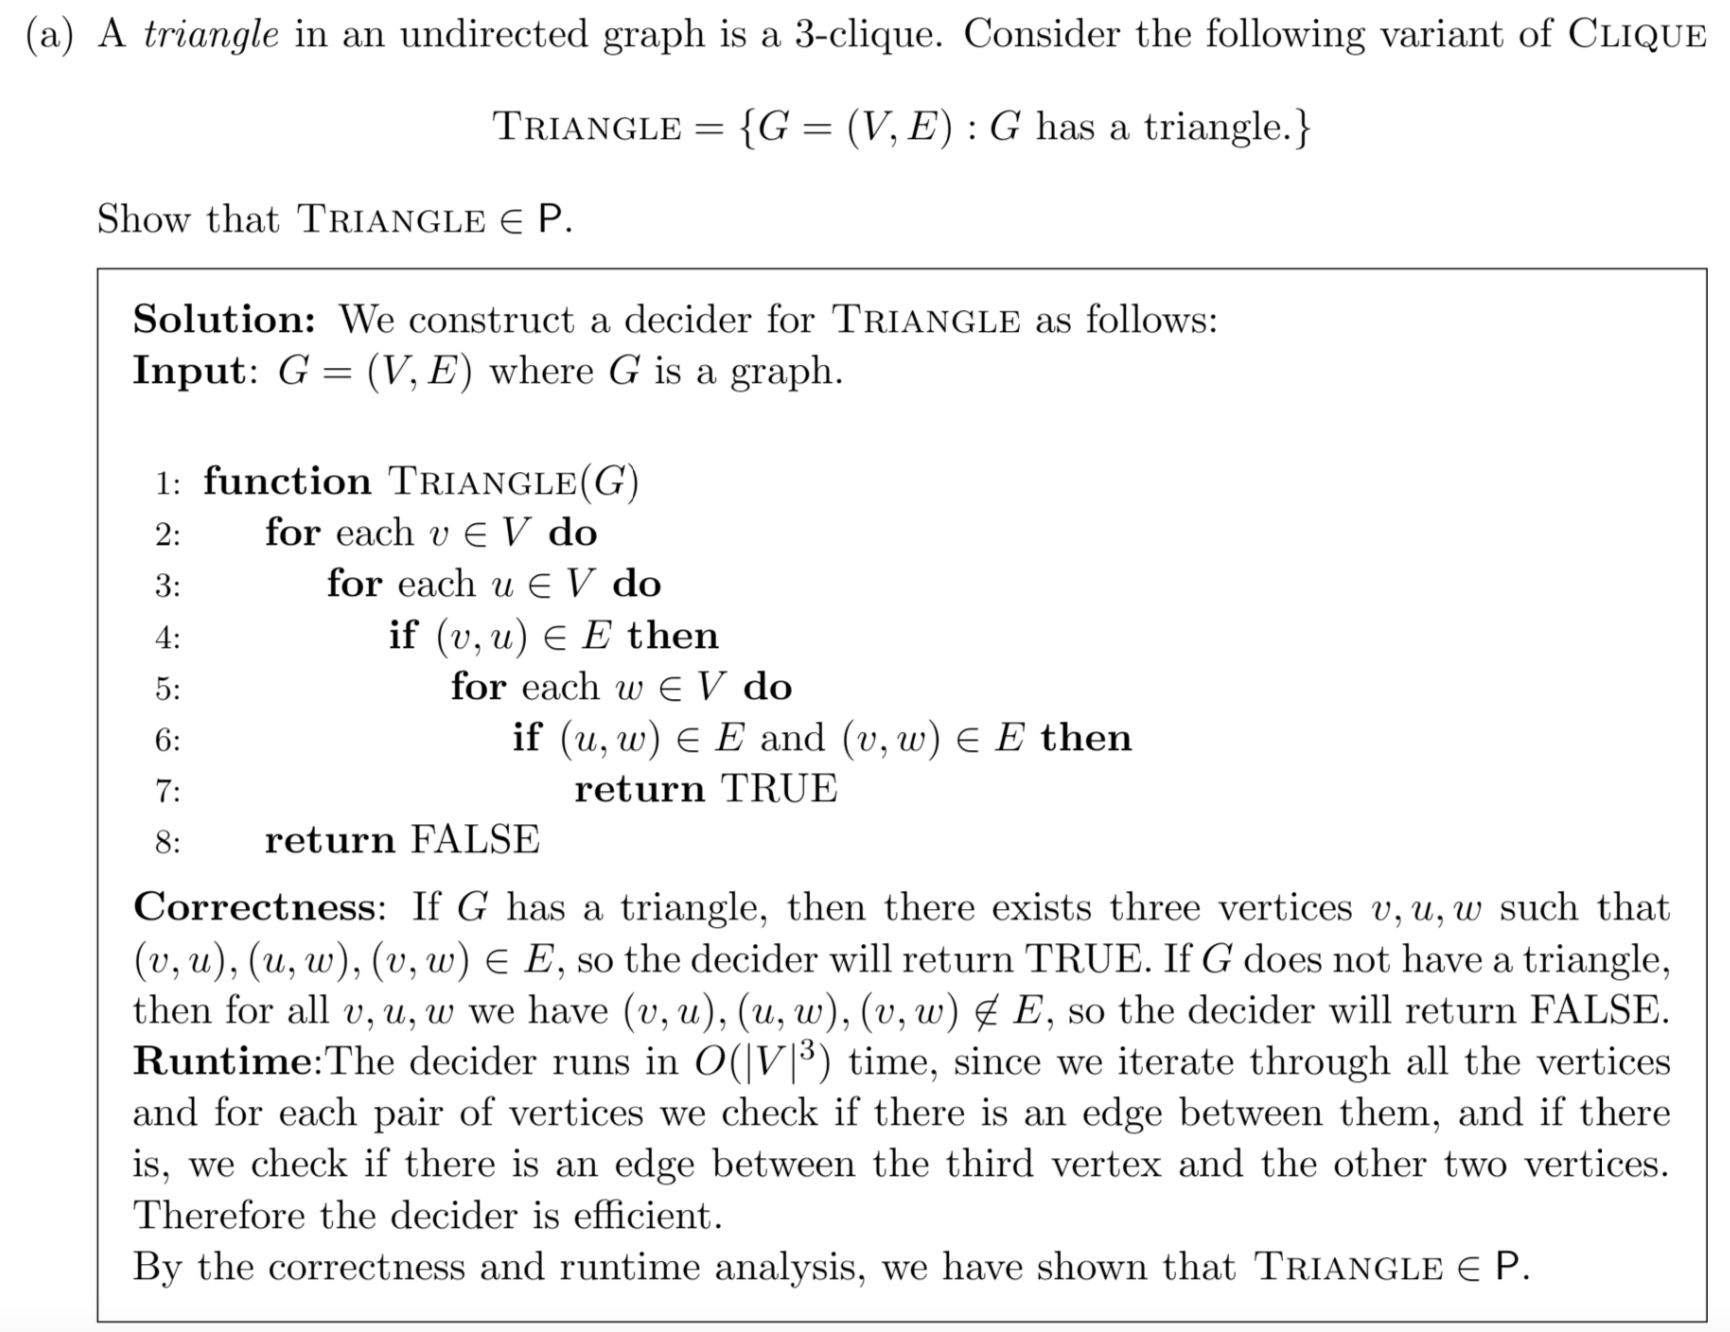
\includegraphics[scale=0.35]{1.png}\\
    \end{center}
    My running time analysis on this question has problem. As we can see, the algorithm involves three layers of loops on $V$, but every iteration involves checking whether two vertices form an edge in $E$ . So every iteration searchs at most the whole $E$, the actual running time is $O(|V|^3|E|)$.
    \end{solution}

    \question \textbf{Warm-up: Multiple Choice.} 
    
    For (a) and (b), select \textbf{the one} correction option. For (c), select \textbf{all} correct options. While justification is \textbf{not required} for full credit, providing it is highly encouraged. \textit{Note: If you are editing the \LaTeX \ file, change} \texttt{choice} \textit{to} \texttt{CorrectChoice} \textit{to fill in the bubble.}
    
    \begin{parts}
    \part [3]  Suppose that there is a randomized algorithm for SAT problem that always output False if there is no satisfying assignment,
    and output True with probability $\ge 0.6$ if there is a satisfying assignment.
    What is the minimum number of False to guarantee that there is no satisfying assignment with at least $98\%$ confidence?
    Assume that the results of each output is independent of all the others.

    \begin{checkboxes}
        \choice 6
        \choice 4
        \choice 2
        \choice 3
        \CorrectChoice 5
    \end{checkboxes}
    
    \begin{solution}

    \end{solution}

    \part [3] Suppose that~$X$ is a non-negative random variable for which $\Ex[X] = 1/2$.
    Select the \textbf{tightest upper bound that \emph{necessarily} holds} for $\Pr[X \geq 5/7]$.
    
    \begin{checkboxes}
        \choice $e^{-(3/14)^2}$
        \CorrectChoice $7/10$
        \choice $5/7$
        \choice $1$
    \end{checkboxes}

    \begin{solution}

    \end{solution}

    \part [5] Suppose $A$ and $B$ are maximization problems, $A \leq_p  B$ and $B \leq_p A$. Select all statements that are true?

    \begin{checkboxes}
        \choice If there is an efficient 0.9 approximation algorithm for $A$, then there is an efficient 0.9 approximation algorithm for $B$.
        \CorrectChoice If there is an efficient algorithm for $A$, then there is an efficient algorithm for $B$.
        \choice If there is an efficient 0.9 approximation algorithm for $A$, then there is an efficient $\alpha$ approximation algorithm for $B$ for some $\alpha < 1$.
        \choice If there is no efficient 0.9 approximation algorithm for $A$, then there is no efficient 0.9 approximation algorithm for $B$.
        \CorrectChoice If there is an efficient algorithm for $A$, then there is an efficient 0.9 approximation algorithm for $B$.
    \end{checkboxes}

    \begin{solution}

    \end{solution}
    
    \end{parts}
    

    \question [15] \textbf{Delivery Route.}

    You are starting a new job as a delivery driver for WindowWalk in Ann Arbor, and they have loaned you an electric car for making deliveries. Each night, you need to charge the car so that it has sufficient power to complete a delivery route, but you don't know the exact route until the next morning. However, you do know the following:
    \begin{itemize}
        \item The route does not visit the same location more than once, except that it begins and ends at your home. We refer to such a route as a \emph{delivery route from your home}.
        \item If your route takes you past a charging station, you can also charge your car on the way.
    \end{itemize}
    Your goal is to charge your car each night to a sufficient level so that it can make it through any delivery route that does not pass a charging station.

    Formally, you model the problem as an unweighted, undirected graph $G$, with vertices as locations in the city and edges as connections between the locations. Given a start vertex $s$ and a set of charging stations $A$, you want to find the maximal delivery route (the route with the highest number of edges) from $s$ that does not go through any of the vertices in $A$. The decision problem is as follows:
    
    \begin{align*}
        \DeliveryRoute = \{(G = (V, E), A, s, k) :~ &G \text{ has a delivery route from $s$ of length exactly $k$}\\
        &\text{that does \textbf{not} go through any vertex in $A\subseteq V$}\}
    \end{align*}

    Given an efficient decider for $\DeliveryRoute$, design and analyze (both correctness and efficiency) an efficient algorithm that given $(G, A, s)$, finds the actual ordered sequence of edges that comprise a delivery route of maximal length from $s$ that does not go through any vertex in $A$. \textit{Hint:} First determine the maximal length.

    \begin{solution}
    \\
\textbf{(1) Determine the Maximal Length of the Delivery Route}
\begin{algorithm}[H]
    \begin{algorithmic}[1]
      \Function{$MaxLength$}{$G, A, s$}
          \State max = 0
          \For{$k$ from 1 to $|E|$}
              \If{$\DeliveryRoute(G, A, s, k)$}
                  \State max = k
              \EndIf         
          \EndFor
          \State \Return max
      \EndFunction
    \end{algorithmic}
    \end{algorithm}
\textbf{(2)Find all only necessary vertices in a delivery route}\\
We use the max returned by $MaxLength$ to find the actual ordered sequence of edges that comprise a delivery route.
\begin{algorithm}[H]
    \begin{algorithmic}[1]
      \Function{$FindVertices$}{$G, A, s, k$}
          \State make a copy of $G$ as $G'$
          \For{$v$ in $V$}
            \State remove $v$ from and its associated edges in $G'$ as $G_{reduced}$
              \If{$\DeliveryRoute(G_{reduced}, A, s, k)$ returns true}
                  \State remove $v$ from and its associated edges in $G'$
              \EndIf        
          \EndFor
          \State \Return $G'$
      \EndFunction
    \end{algorithmic}
    \end{algorithm}

\textbf{(3)Find the actual ordered sequence of edges that comprise a delivery route}
\\We use the $G'$ returned by $FindVertices$ and the $max$ returned by $MaxLength$ as $k$, as an input to the new function. $G' = (V', E')$ now contains all the necessary vertices for the delivery route. Now we delete edges to make $G'$ only contains a cycle.
\begin{algorithm}[H]
    \begin{algorithmic}[1]
      \Function{$FindRoute$}{$G' = (V',E'), A, s, k$}
          \State $route = [s]$
          \For {$e$ in $E'$}
            \State remove $e$ from $E'$
            \If{$\DeliveryRoute(G', A, s, k)$ returns true}
                \State continue
            \Else
                \State restore $e$ in $G'$
            \EndIf
          \EndFor 

          \State loop V' to find a vertice $v_0$ that is connected to s
          \Comment Now the $G'$ only contains a cycle, which means that every vertex in $V'$ is connected to two other vertexs in $V'$.
          \State currentVertex = $v_0$
          \State lastVertex = $s$
          \State loop through the $V'$ to find the next vertex in the cycle, and add next vertex into $route$, until current vertex is $s$.

          \State \Return $route$
      \EndFunction
    \end{algorithmic}
    \end{algorithm}
\textbf{(4) Correctness Justification}\\
1. Note that $k$ is an integer since the graph is unweighted, and is bounded by the size of $E$, so by iterating from 1 to $|E|$, we can find the maximal length of the delivery route using the $MaxLength$ function.

2. By the $FindVertices$ function, the returned graph $G'$ contains all the and only the necessary vertices for the delivery route, since if a vertex is unnecessary, then $G_{reduced}, A, s, k$ returns true and it will be deleted, and since $k$ is the maximal length, if a vertex is necessary in the route, $G_{reduced}, A, s, k$ will return false so it will not be deleted. 

3. Likewise, $FindRoute$ delete all unnecessary cycles and leaves only a cycle in $G'$, and then find the actual ordered sequence of edges that comprise a delivery route by looping through the vertices in the cycle.\\
\textbf{(5) Efficiency Analysis}\\
Suppose the runtime of $DeliveryRoute$ function is $P$ which is a polynomial to the input G, then the runtime of $MaxLength$ is $O(|E|P + |V|P + |E|P +|V|) = O((|E|+|V|)P)$, which is a polynomial to the input, so the search algorithm is efficient if the $DeliveryRoute$ function is efficient.
    \end{solution}

    \question \textbf{Approximate $\fSetCov$.}

    In this question, you will consider a variant of the $\SetCov$ problem where each element of the universe is in a limited number of subsets.
    Formally, in the $\fSetCov$ problem, we are given a ``universe'' (set)~$U$ and subsets $S_1, \ldots, S_n \subseteq U$ \emph{where each universe element appears in at most~$f$ of the subsets}.
    The goal is to find a smallest collection of the subsets that ``covers''~$U$, i.e., an $I \subseteq \set{1,\ldots,n}$ of minimum size such that $\bigcup_{i \in I} S_{i} = U$.
    We assume that $\bigcup_{i=1}^{n} S_{i} = U$, otherwise no solution exists.

    You will analyze an approximation algorithm ``$f$-cover'' for the $\fSetCov$ problem.
    The algorithm is a generalization of the ``double cover'' algorithm for $\VertCov$ from lecture, and it works essentially as follows: while there is some uncovered element~$u$ in the universe, add to the cover \emph{all} the subsets to which~$u$ belongs.
    The formal pseudocode is as follows.
    The notation $I(u) = \set{i : u \in S_i}$ for $u \in U$, that is, $I(u)$ indicates the subsets to which~$u$ belongs.

    \begin{algorithm}[H]
    \begin{algorithmic}[1]
      \Function{$f$-cover}{$U, S_1, \ldots, S_n$}
          \State $I = C = \emptyset$
          \Comment{selected indices $I$, covered elements $C$}
          \While{$C \neq U$}
              \Comment{not all elements are covered}
              \State choose an arbitrary $u \in U \setminus C$
              \label{fcov:pickuncovered}
              \Comment{element $u$ is not yet covered}
              \State $I = I \cup I(u)$, $C = C \cup \bigcup_{i \in I(u)} S_{i}$
              \Comment{add \emph{all} subsets $S_{i}$ containing $u$ to the cover}
          \EndWhile
          \State \Return $I$
      \EndFunction
    \end{algorithmic}
    \end{algorithm}
    
    Fix some arbitrary $\fSetCov$ instance, and let~$I^*$ denote an optimal set cover for it.
    Let~$E$ denote the set of elements~$u$ chosen in Step~\ref{fcov:pickuncovered} during an execution of the algorithm, and let~$I$ denote the algorithm's final output.

  \begin{parts}
    \part[4] Prove that $I(u) \cap I(u') = \emptyset$ for every distinct $u, u' \in E$.
    In other words, prove that if $u$ and $u'$ are each selected as the uncovered element in different iterations, none of the $S_i$ contains both~$u$ and~$u'$.
    \label{it:fsc-one}
        
    \begin{solution}
    Suppose an element \( u \) is chosen in the algorithm, then all subsets containing \( u \) are added to the set cover. 
    \\Suppose another element \( u' \) is selected in a subsequent iteration, it implies that \( u' \) was not covered previously. Thus, there is no subset that contains both \( u \) and \( u' \), implying that \( I(u) \cap I(u') = \emptyset \).
    \end{solution}

    \part[4] We want a lower bound on $\text{OPT} = |I^*|$.
    Using the previous part, prove that $|E| \leq |I^*|$.
    
    \begin{solution}
    Each element \( u \in E \) chosen by the algorithm must be covered by at least one subset in any feasible solution. Since \( I(u) \cap I(u') = \emptyset \) for all \( u \neq u' \), each element \( u \in E \) provides a unique contribution to the cover. Hence, the number of elements in \( E \) sets a lower bound on the number of subsets required in an optimal solution, implying \( |E| \leq |I^*| \).

    \end{solution}
    
    \part[4] We want an upper bound on $\text{ALG} = |I|$.
    Prove that $|I| \leq f \cdot |E|$, and conclude that the $f$-cover algorithm is an $f$-approximation algorithm for the $\fSetCov$ problem.
        
    \begin{solution}
     Each element \( u \) chosen adds at most \( f \) subsets to \( I \), as each element appears in at most \( f \) subsets. Thus, the total number of subsets added to \( I \) is at most \( f \cdot |E| \). Since \( |E| \leq |I^*| \), it follows that \( |I| \leq f \cdot |I^*| \), denoting that the algorithm is an \( f \)-approximation algorithm.

    \end{solution}

    \part[4] Prove that for every positive integer~$f$, there is an input for which the $f$-cover algorithm necessarily outputs a cover that is \emph{exactly} $f$ times as large as an optimal one.
    
    \begin{solution}
     For each positive integer $f$, Consider a universe \( U \) with \( f \) elements and \( n = f \) subsets, where each subset \( S_i = \{u_i\} \). Each element appears in exactly one subset, so the \( f \)-cover algorithm will select all subsets when the first element is picked, resulting in \( |I| = f \). This is a case where the output of \( f \)-cover is exactly \( f \) times the size of an optimal solution.
    \end{solution}
  \end{parts}

  \question \textbf{Indicator variables and linearity of expectation.}

  Let $n$ be a positive integer and $0 < p < 1$.
  Let $G_{n, p}$ denote a random undirected graph on~$n$ vertices, constructed as follows: for each (unordered) pair of distinct vertices $u, v \in V$, include the edge $(u, v)$ in $G_{n, p}$ with probability~$p$, independently of all other random choices.
  
  \begin{parts}
    \part[5] Derive the expected number of edges in $G_{n, p}$.
    
    \begin{solution}
The total number of pairs of vertices between \( n \) vertices is \( \binom{n}{2} \), so the expected number of edges \( \Ex[E] \) is:

\[ \Ex[E] = \binom{n}{2} \cdot p = \frac{n(n-1)}{2} \cdot p \]
    \end{solution}
    
    \part[5] Derive the expected degree of any vertex in $G_{n, p}$.
    
    \begin{solution}
  Each vertex \( v \) can potentially connect to \( n-1 \) other vertices, each edge formed independently with probability \( p \).
  Fix a vertex $v \in V$, and let $d_v$ denote the degree of vertex $v$.
  Consider the indicator variable $X_{uv}$ for whether vertex $u,v \in V$ is connected.
  So the expected degree of vertex \( v \) is:


\[ \Ex[d_v] = \sum_{u \in V-{v}} \Ex[X_{uv}] = (n-1) \cdot p \]
    \end{solution}
    
    \part[4] A \emph{triangle} in a graph is a set of three (distinct) vertices that have an edge between every pair of them.
    Derive the expected number of triangles in $G_{n,p}$.
    
    \begin{solution}
The number of ways to choose three vertices from \( n \) is \( \binom{n}{3} \).
For each triplet of vertices \( (u, v, w) \), the probability that all three possible edges among them are present is \( p^3 \), by independency.
Therefore, the expected number of triangles \( \Ex[T] \) is:

\[ \Ex[T] = \binom{n}{3} \cdot p^3 = \frac{n(n-1)(n-2)}{6} \cdot p^3 \]  \[(n \geq 2)\].
    
    \end{solution}
      
    \part[4] Prove that the number of triangles in $G_{n,p}$ is at least $n^3 p^2$ with probability at most $p/6$.

    \begin{solution}
By Markov's inequality: \( \Pr[T \geq x] \leq \frac{\Ex[T]}{x} \).
\\Therefore for \( x = n^3 p^2 \):
\[ \Pr[T \geq n^3 p^2] \leq \frac{\frac{n(n-1)(n-2)}{6} \cdot p^3}{n^3 p^2} = \frac{(n-1)(n-2)}{6n^2} \cdot p \leq \frac{p}{6}\] since $0 \leq (n-1)(n-2) \leq n^2$ for $n \geq 2$.
    \end{solution}
  \end{parts}

  \question \textbf{Randomized max-cut.}
  
  In this problem, all graphs are undirected and (as usual) have \emph{no self-loops}, i.e., there is no edge from a vertex to itself.
  For a cut $S \subseteq V$ in a graph $G=(V,E)$, let $C(S) \subseteq E$ denote the subset of edges ``crossing'' the cut, i.e., those that have exactly one endpoint in~$S$.
  The size of the cut is then $\abs{C(S)}$.
  Consider the following randomized algorithm that outputs a cut in a given graph $G=(V,E)$.

    \begin{algorithm}[H]
      \begin{algorithmic}[1]
        \State initialize $S = \emptyset$
        \ForAll{$v \in V$}
        \State put $v$ into $S$ with probability 1/2, independently of all others
        \EndFor
        \State \Return $S$
      \end{algorithmic}
    \end{algorithm}    
  
  \begin{parts}
    \part[5] Define suitable indicator variables and use linearity of expectation to prove that \emph{in expectation}, the above algorithm obtains a $1/2$-approximation for $\MaxCut$.
    That is, the expected size of the output cut is at least half the size of a maximum cut.
    
    \begin{solution}\\
Let \( I_{uv} \) be an indicator variable that is 1 if edge \( \{u, v\} \) crosses the cut \( S \), and 0 otherwise. The edge crosses the cut if exactly one of its endpoints is in \( S \). Each vertex is added to \( S \) independently with probability \( \frac{1}{2} \), so:
\[ \Pr[I_{uv} = 1] = \Pr[u \in S, v \notin S] + \Pr[u \notin S, v \in S] = \frac{1}{2} \cdot \frac{1}{2} + \frac{1}{2} \cdot \frac{1}{2} = \frac{1}{2} \]

The expected size of the cut \( |C(S)| \) is:
\[ \Ex[|C(S)|] = \sum_{\{u, v\} \in E} \Ex[I_{uv}] = \frac{|E|}{2} \]
Since the size of a maximum cut \( |E_{max}| \leq \frac{|E|}{2} \), the algorithm achieves a \( \frac{1}{2} \)-approximation in expectation:
\[ \Ex[|C(S)|] \geq \frac{1}{2} |E_{max}| \]
    \end{solution}
      
    \part[5] Prove that $\Pr[|C(S)| \geq (1-\epsilon)|E|/2] \geq \frac{\epsilon}{1+\epsilon}$ for any $\epsilon > 0$.
  
    Notice that for $\epsilon = 1/(2|E|)$, this is a lower bound on the probability that the number of edges crossing~$S$ is at least $|E|/2$, because the number of crossing edges is an integer.

    \begin{solution}
We prove it by applying reverse Markov's inequality to the expected number of crossing edges: $C(S) \leq |E| $ for all cuts $S$, so we can set $b = |E|$.
\\Then by the reverse Markov's inequality:
\begin{align*}
    \Pr[|C(S)| \geq (1-\epsilon)|E|/2] &\geq \frac{\Ex[|C(S)|] - (1-\epsilon |E|/2)}{|E| - (1-\epsilon)|E|/2} \\
    &= \frac{|E|/2 - (1-\epsilon |E|/2)}{|E| - (1-\epsilon)|E|/2} \\  
    &= \frac{\epsilon|E|/2}{(1+\epsilon)|E|/2} \\ 
    &= \frac{\epsilon}{1+\epsilon}
\end{align*}
    \end{solution}

    \part[5] As a stepping stone to the next part, we consider the following intermediate question.
    
    Consider a probability experiment that consists of a sequence of ``attempts,'' where each attempt succeeds with probability~$p$, independently of all others.
    We keep making attempts until one succeeds, at which point the experiment terminates.

    Let~$X$ denote the number of attempts until termination (including the attempt that finally succeeds).
    Prove that
    \[ \Ex[X] = p + (1-p)(1+\Ex[X]) \; \text, \] and conclude that $\Ex[X] = 1/p$.
    (The distribution of~$X$ is known as the \emph{geometric distribution} with success probability $p$.)

    \begin{solution}
Let \(X\) denote the number of attempts until termination (including the attempt that finally succeeds), and let each attempt succeed with probability \(p\), independently of the others.

Consider the outcomes of the first attempt:\\
\textbf{Case 1: Success on the First Attempt:} This occurs with probability \(p\). If the first attempt is successful, \(X = 1\).\\
\textbf{Case 2: Failure on the First Attempt:} This occurs with probability \(1-p\). If the first attempt fails, the number of additional attempts required would still be expected to be \(\mathbb{E}[X]\). Since this includes the failed first attempt, the total expected number of attempts would then be \(1 + \mathbb{E}[X]\).

So the total expected value of \(X\) is:
\[
\mathbb{E}[X] = p \cdot 1 + (1-p) \cdot (1 + \mathbb{E}[X])
\]


To solve for \(\mathbb{E}[X]\), rearrange and isolate \(\mathbb{E}[X]\) on one side:
\[
\mathbb{E}[X] = p+1-p+ (1-p)\mathbb{E}[X] = 1 + (1-p)\mathbb{E}[X]
\]
\[
1-(1-p)\mathbb{E}[X] = 1
\]
\[
\mathbb{E}[X] = {1\over p}
\]

    \end{solution}
 
    \part[5] Suppose we repeatedly run our randomized $\MaxCut$ algorithm until we get a cut of size at least $|E|/2$.
    Derive an upper bound on the expected number of attempts that are needed.

    \begin{solution}
     Given each attempt to obtain a cut of size at least \( \frac{|E|}{2} \) succeeds with a probability \( \frac{1}{2} \):
\[ \Ex[\text{Attempts}] = 1/p \leq \frac{1}{1/2} = 2 \]
So an upper bound on the expected number of runs of the algorithm to achieve a cut of at least \( \frac{|E|}{2} \) is 2.

    \end{solution}
  \end{parts}

\question \textbf{Cryptography.}

\begin{parts}
    \part [6] Alice and Bob agree on the prime $p = 17$ and generator $g = 6$, and wish to establish a shared secret key $k$ using the Diffie-Hellman protocol. 
    
    Suppose Alice privately chooses $a=3$ and Bob privately chooses $b=12$.  What is Alice's message to Bob?  What is Bob's message to Alice?  What is the secret key $k$?

    \begin{solution}
    \\
    \textbf{Alice's message to Bob:}
    \[ g^a \equiv 6^3 \equiv 2 \cdot 6 \equiv 12 \mod 17 \]
    So Alice's message to Bob is 12.

     \textbf{Bob's message to Alice:}
    \[ g^b \equiv 6^{12} \equiv (6^3)^4 \equiv (144)^2 \equiv 8^2 \equiv 13 \mod 17\]
    So Bob's message to Alice is 13.

     \textbf{Shared secret key \( k \):}
    \[ 12^{12} \equiv 13^3 \equiv 4 \mod 17\]
    So, the shared secret key \( k \) is 4.
    \end{solution}

    \part [4] Alice uses modulus $n = 65$ and RSA public key $e = 29$.
    Determine a possible private key $d$ and calculate Alice's RSA-signature for the 
    message $m=3$.

    \begin{solution}
    \\
    \( n = 65 = 5 \times 13, \; \phi(65) = (5-1)(13-1) = 48 \)\\
\textbf{Finding a private key \( d \):}\\
    Since $e=29$, we solve \( 29\,d \equiv 1 \mod 48 \).\\
    Using the extended Euclidean algorithm, \( d = 5 \).
    \[ 29 \cdot 5 \mod 48 = 1 \]
So a private key \( d \) is 5.\\
\textbf{RSA Signature for \( m = 3 \):}
    \[ s \equiv m^d \equiv 3^5 \equiv 48 \mod 65 \]
    So the RSA signature \( s \) is 48.
    \end{solution}
    \end{parts}
    \end{questions}


\end{document}